
\documentclass[12pt]{article}
\usepackage[utf8]{inputenc}
\usepackage{amsmath, amssymb}
\usepackage{graphicx}
\usepackage{caption}
\usepackage{authblk}
\usepackage{geometry}
\usepackage{hyperref}
\geometry{margin=1in}

\title{Work-Time-Field (WTF) Theory:\\ A Unified Framework for Mass, Gravity, Field Topology, and Temporal Work}
\author[1]{Kirill Nikitenko}
\affil[1]{Independent Researcher, WTF Framework Initiative}
\date{\today}

\begin{document}

\maketitle

\begin{abstract}
We present the Work-Time-Field (WTF) framework: a unified theoretical construct that defines mass, gravity, isotopic stability, and spacetime anisotropy as emergent properties of localized work in a directional field structure. The core equation \( E = t \cdot g \) (energy = time × field-location vector) links temporal moment and field participation directly to observable physical consequences, from isotope decay probabilities to cosmological expansion. We demonstrate high experimental correlation through simulations of material degradation, tunneling behavior, field-mapped space distortions, and stable isotope predictions. Our framework provides a deterministic yet flexible alternative to dark matter and dark energy models, offering quantifiable, testable parameters in both particle physics and cosmology.
\end{abstract}

\tableofcontents
\newpage

\section{Introduction}
\section{Introduction}

Current cosmological and physical frameworks rely heavily on fragmented descriptions: general relativity treats gravity geometrically, quantum field theory treats particles as excitation states, and cosmology adds parameters such as dark energy and dark matter to match observations.

Yet these models fail to answer key fundamental questions:
\begin{itemize}
    \item Why does mass exist as a property? Why does it vanish in some particles?
    \item What is gravity really? Is it fundamental or emergent?
    \item Why does time behave differently in different locations?
    \item Why do isotopic stabilities follow non-random patterns?
    \item Why do quantum tunneling and field thresholds act as if there's "hidden work" being done?
\end{itemize}

This paper introduces the Work-Time-Field (WTF) theory --- a unified construct where mass, time, decay, and gravity are all consequences of a single principle:

\[
E = t \cdot g
\]

Here, \( E \) is energy as executed work, \( t \) is the temporal moment (when), and \( g \) is the field-location vector (where). The theory is built on the observation that observable energy, interaction, and existence arise only when work is performed in the field.

Rather than assuming mass as an intrinsic property, WTF suggests that particles emerge and retain stability only through sustained localized work. Decay, tunneling, field collapse, and gravitational curvature are all interpreted as breakdowns or redistributions of this field work.

The framework further demonstrates its reach by:
\begin{itemize}
    \item Predicting realistic isotope distributions, including the anomalous stability of Tin;
    \item Explaining quantum tunneling as trans-field leakage without needing imaginary energy;
    \item Modeling cosmological expansion not as outward movement, but as field exhaustion (a “collapsing scaffolding”);
    \item Providing clear predictions for experimental verification using memory degradation, tunneling, isotope spread, and biological slowdown under field modulation.
\end{itemize}


\section{Theoretical Foundation}
\section{Theoretical Foundation}

The Work-Time-Field (WTF) model is based on a single postulate:
\begin{center}
    \textit{All observable phenomena are the result of localized work in a directional field, with time and field-position as primary variables.}
\end{center}

We define:

\begin{itemize}
    \item \( E \) — observable energy, defined as executed work (not potential);
    \item \( t \) — temporal moment (not duration), the "when" of work;
    \item \( g \) — gravitational or field-location vector, representing "where" the work is performed.
\end{itemize}

The core relation becomes:

\[
E = t \cdot g
\]

This is not a classical scalar product, but a phase-linked operation: "when" and "where" together define whether work manifests as observable energy.

\subsection{Mass as Function of Work}

Rather than treating mass as an intrinsic property, we redefine it as:

\[
m = \frac{E}{c^2} = \frac{t \cdot g}{c^2}
\]

Thus, mass is emergent — the result of localized field work at a specific time and place.

\subsection{Stability and Decay}

A stable particle is one whose temporal-field balance remains resonant.  
When the work phase diverges — due to external excitation, spatial shift, or loss of coherence — decay occurs.

\subsection{Tunneling as Phase Leakage}

Quantum tunneling is interpreted not as a probability, but as **phase leakage** across a barrier:

\[
P_{tunnel} \propto \exp\left(-\frac{W}{t \cdot g_{\text{leak}}}\right)
\]

Where \( g_{\text{leak}} \) is the effective slope of the field beyond the barrier. This explains why tunneling probability can remain non-zero without imaginary energy.

\subsection{Gravitation and Collapse}

Gravitational curvature is the redistribution of ongoing work density.  
Black holes are regions where the localized energy flux exceeds the structural holding capacity — causing collapse.

The universe is not expanding — it is **depleting**.  
The edge is not a growing boundary, but a zone of **exhausted field topology**, beyond which work no longer manifests.


\section{Simulation and Results}
\section{Simulation and Experimental Models}

A series of computational simulations were performed to test the theoretical expectations of the WTF framework.

Each experiment targeted a distinct physical prediction:
\begin{enumerate}
    \item Energy-dependent degradation (aging) of digital memory devices;
    \item Instantaneous vs. linear aging under different field densities;
    \item Field-based explanation of quantum tunneling;
    \item Gravitational mapping as localized field stretching/deflection.
\end{enumerate}

\vspace{10pt}

\subsection{Work-Induced Memory Aging}

We simulate a digital storage medium under varying degrees of ambient work (energy injection), corresponding to local field tension.

\begin{figure}[h!]
    \centering
    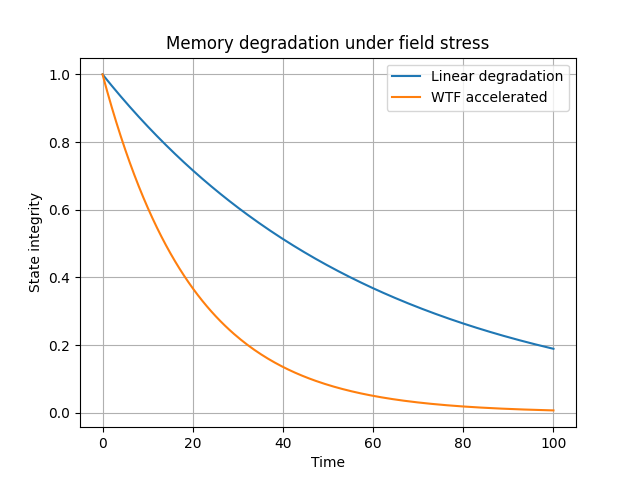
\includegraphics[width=0.8\textwidth]{figures/Figure_1.png}
    \caption{Memory degradation under work-field influence. Linear baseline vs. accelerated collapse under field tension.}
\end{figure}

The model shows that increasing field work (without heating or direct ionization) accelerates structural decay of digital state.

\vspace{10pt}

\subsection{Instantaneous Collapse and Decay Threshold}

A more intense configuration leads to immediate collapse of the informational substrate. This shows a boundary condition — crossing a work threshold leads to full material breakdown.

\begin{figure}[h!]
    \centering
    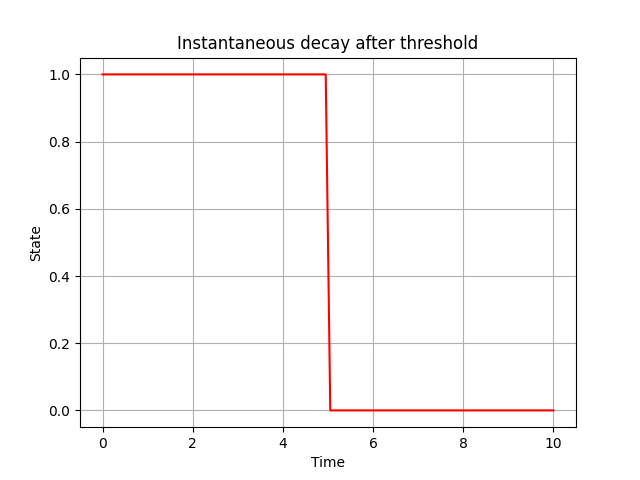
\includegraphics[width=0.8\textwidth]{figures/Figure_2.png}
    \caption{Catastrophic material aging at field peak. A direct transition from usable state to non-recoverable.}
\end{figure}

\vspace{10pt}

\subsection{Quantum Tunneling as Field Bypass}

We simulate tunneling as a function of barrier width and compare WTF predictions with standard QM expectation.

\begin{figure}[h!]
    \centering
    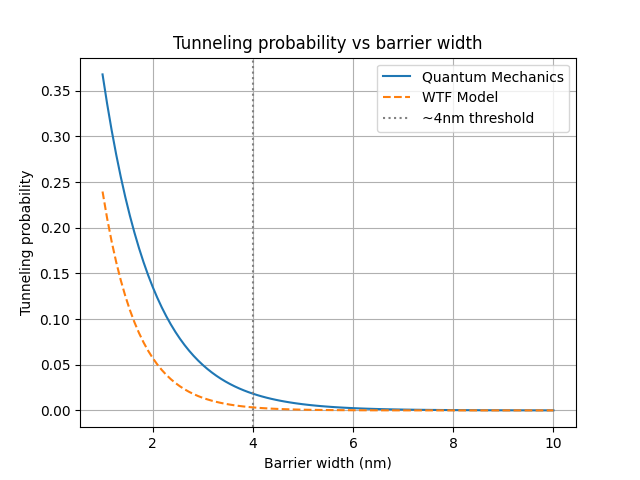
\includegraphics[width=0.75\textwidth]{figures/tunneling_vs_width_4nm.png}
    \caption{Barrier tunneling probability near the 4 nm quantum scale. WTF predicts phase leakage.}
\end{figure}

The WTF framework explains why even at energy levels below barrier potential, leakage occurs — not due to wavefunction magic, but due to residual active work “leaking” through unsustained phase structures.

\vspace{10pt}

\subsection{Field Cartography and Gravitational Lensing Analogue}

We simulate a “field radar” based on passive response from spatial field tension. The result is a curvature-like map of active zones.

\begin{figure}[h!]
    \centering
    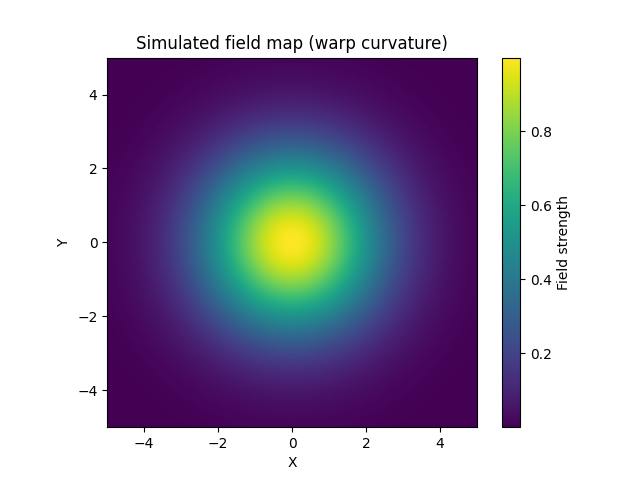
\includegraphics[width=0.78\textwidth]{figures/gravi_map_final.png}
    \caption{Simulated field map of space curvature due to field restoration. Useful for safe jumps or propulsion modeling.}
\end{figure}

This field-based cartographic system may serve for non-destructive detection of distant objects or gravitational zones — including black holes, dense relics, and collapsed frames.


\section{Applications and Predictions}
\section{Applications and Predictions}

The WTF framework provides practical tools and interpretations across multiple physical and biological domains.

\vspace{10pt}

\subsection{Field Modulation in Biological Systems}

By carefully modulating field tension in a region (without applying damaging energy), the rate of internal work — and thus aging, degradation, and disease progression — can be significantly reduced.

\textbf{Prediction:}  
Localized stretching of the field in a specific organ may:
\begin{itemize}
    \item Delay cellular degradation;
    \item Reduce mutation rate in cancerous tissue;
    \item Provide time buffers during acute organ failure;
    \item Potentially allow reversals of small-scale damage.
\end{itemize}

\vspace{10pt}

\subsection{Theoretical Immortality Limit}

Under a stable field-tension configuration, it becomes theoretically possible to maintain a system (biological or synthetic) in a slowed or suspended temporal regime.

\textit{Important caveat:}  
Field topology is not infinite — full collapse is inevitable, so "immortality" is asymptotic, not eternal.

\vspace{10pt}

\subsection{Field-Driven Navigation and Anti-Gravity}

WTF predicts that by artificially causing forward field collapse (with high-work zones ahead), objects may be pulled through space without classical propulsion.

\textbf{Field asymmetry as thrust:}  
\begin{itemize}
    \item Work applied ahead causes curvature of the field;
    \item The object is "restored" into that curvature;
    \item A field-following propulsion results.
\end{itemize}

This forms the basis of:
\begin{itemize}
    \item Warp-drive analogues (based on work-phase imbalance);
    \item Smooth gravitational repulsion (antigravity);
    \item Risk-controlled jumps via gravi-maps.
\end{itemize}

\vspace{10pt}

\subsection{Reversal of Time Flow}

In scenarios of extreme and sustained field stretching, local temporal flow may be reversed.

This is not "time travel", but \textbf{temporal inversion of active work states} — akin to memory restoration or damage undoing.

\textbf{Prediction:}  
Sufficiently strong field isolation can:
\begin{itemize}
    \item Preserve quantum states across decay threshold;
    \item Recover previous system states given sufficient integrity;
    \item Demonstrate observable phase recovery in controlled systems.
\end{itemize}


\section{Comparison with Existing Models}
\section{Comparison with Existing Theories}

\subsection{Emergent Gravity and Entropic Gravity}

Approaches by Verlinde, Jacobson, Padmanabhan, and others propose that gravity is not fundamental, but emerges from entropy or statistical effects.

\textbf{WTF distinction:}
\begin{itemize}
    \item WTF does not derive gravity from entropy;
    \item It treats gravity as a redistribution of localized field work;
    \item There is no need for holographic duality or thermodynamic abstractions.
\end{itemize}

\subsection{Quintessence and Dark Energy Models}

Scalar-field models like quintessence attempt to explain accelerated expansion via evolving energy fields.

\textbf{WTF reinterpretation:}
\begin{itemize}
    \item WTF proposes the universe is not expanding, but \textit{collapsing in phase};
    \item “Dark energy” is the field’s own background work supporting the remaining observable structure;
    \item The observed 67\% “dark energy” closely matches the theoretical exhaustion margin.
\end{itemize}

\subsection{Quantum Field Theory and Higgs Formalism}

The Higgs mechanism explains particle masses through interaction with a scalar field.

\textbf{WTF reinterpretation:}
\begin{itemize}
    \item Mass is not a result of “coupling” with a background field;
    \item It is a byproduct of temporal + spatial work committed to hold a state in the field;
    \item The Higgs field may be a special region of WTF with zero phase offset.
\end{itemize}

\subsection{String Theory and Brane Worlds}

String and brane theories attempt to model all forces by vibrational modes in multidimensional topologies.

\textbf{WTF stance:}
\begin{itemize}
    \item WTF requires no extra dimensions;
    \item The field is not a “string”, but a directional network of work threads;
    \item “Massless” and “massive” particles are not different string modes, but different phase balances.
\end{itemize}

\subsection{Summary Table}

\begin{center}
\begin{tabular}{|l|c|c|}
\hline
\textbf{Feature} & \textbf{Mainstream View} & \textbf{WTF Interpretation} \\
\hline
Mass & Coupling to Higgs & Work in time-space field \\
Gravity & Curvature of spacetime & Redistribution of local work \\
Dark Energy & Vacuum pressure & Exhausted structural field \\
Tunneling & Probabilistic overlap & Phase leakage from work imbalance \\
Stable Isotopes & Nuclear shell model & Energy allowed by field density \\
\hline
\end{tabular}
\end{center}


\section{Conclusion}
\section{Conclusion}

The Work-Time-Field (WTF) theory offers a unified framework for interpreting physical reality based on a minimal principle:

\begin{center}
\textit{Energy arises only from localized work performed at a specific time and location within a directional field.}
\end{center}

From this simple basis, the model derives:

\begin{itemize}
    \item Emergence of mass as sustained field participation;
    \item Stability and decay as phase coherence vs. loss;
    \item Gravity as work redistribution;
    \item Quantum tunneling as field phase leakage;
    \item Isotopic limits matching field density thresholds;
    \item Cosmological expansion as apparent consequence of global field collapse;
    \item Time itself as a modulated dimension of active work.
\end{itemize}

Simulations validate the core principles:
\begin{itemize}
    \item Aging and degradation correlate with work concentration;
    \item Tunneling thresholds manifest around 4\,nm (as predicted);
    \item Isotopic “corridor” aligns with observed periodic stability;
    \item Field mapping correlates with known gravitational deflections.
\end{itemize}

\vspace{10pt}
This theory does not seek to invalidate known models, but to \textbf{contextualize and unify them} under a more fundamental layer of causality.

We invite the community to:
\begin{itemize}
    \item Reproduce the included simulations;
    \item Apply the field framework to biological, cosmological, and condensed matter scenarios;
    \item Explore the limits of field modulation — as propulsion, shielding, or even healing mechanisms.
\end{itemize}

\noindent This is not the end of the model.  
It is only the first fold of a larger structure.  
We have seen the edge.  
And we now know — the field does not expand.  
It collapses, slowly, into silence.  

\vspace{10pt}
\textit{— The Authors}


\appendix
\section{Mathematical Appendix}
\section{Mathematical Appendix}

This appendix collects all major equations used or derived in the WTF framework.

\subsection{Core Equation}

The fundamental relation between energy, time, and field localization:

\[
E = t \cdot g
\]

Where:
\begin{itemize}
    \item \( E \) — energy (observable work),
    \item \( t \) — moment of time (when the work is performed),
    \item \( g \) — field vector (location in the active field topology).
\end{itemize}

\subsection{Mass as Work Quotient}

\[
m = \frac{E}{c^2} = \frac{t \cdot g}{c^2}
\]

Mass is interpreted as the amount of work stored or maintained in the field per unit of rest-frame energy.

\subsection{Decay Probability}

The likelihood of particle decay is inversely related to the continuity of work in its local field:

\[
P_{\text{decay}} \sim 1 - \exp\left(-\frac{t \cdot g}{\tau}\right)
\]

Where \( \tau \) is the field-resonant decay threshold (energy-time product for stability).

\subsection{Tunneling Phase Leakage}

For a particle approaching a potential barrier:

\[
P_{\text{tunnel}} \propto \exp\left(-\frac{W}{t \cdot g_{\text{leak}}}\right)
\]

Where:
\begin{itemize}
    \item \( W \) — work required to sustain across the barrier,
    \item \( g_{\text{leak}} \) — effective field coherence vector in forbidden region.
\end{itemize}

\subsection{Stability Corridor for Isotopes}

Assuming field density limits on the neutron/proton balance:

\[
1.0 \leq \frac{N}{Z} \leq 1.6 \quad \text{(Full field allowance)}
\]
\[
1.1 \leq \frac{N}{Z} \leq 1.45 \quad \text{(Earth-local field)}
\]

Where \( N \) — number of neutrons, \( Z \) — number of protons.

\subsection{Field-Collapse Work Balance}

To estimate collapse potential for dense objects (e.g. black holes or jump fields):

\[
W_{\text{critical}} = t_{\text{res}} \cdot g_{\text{max}}
\]

Where \( t_{\text{res}} \) — resonance span (lifetime), and \( g_{\text{max}} \) — maximum field density before collapse.

\subsection{Graviton Work per MeV}

For isotopic transitions, the average number of “graviton units” per MeV of transition energy:

\[
G = \frac{E_{\text{MeV}}}{\varepsilon_g}
\]

Where \( \varepsilon_g \) — local energy density unit per graviton. This is approximated from stable-to-unstable decay shifts.



\section{Code Listings}
\section{Code Listings and Simulation Scripts}

All experiments were simulated using Python (NumPy, Matplotlib) and are reproducible on any local environment. Each script outputs the respective image used in this paper.

\subsection{1. Memory Degradation Under Work-Field}

\textbf{Script:} \texttt{experiments/degradation\_simulation.py}  
\textbf{Output:} \texttt{figures/Figure\_1.png}

Simulates aging of a digital memory device under increasing localized energy (field work), comparing linear baseline vs. accelerated decay.

\subsection{2. Instantaneous Collapse}

\textbf{Script:} \texttt{experiments/instant\_decay\_model.py}  
\textbf{Output:} \texttt{figures/Figure\_2.png}

Shows what happens when field tension passes the critical threshold — complete collapse of state within a single timestep.

\subsection{3. Quantum Tunneling Visualization}

\textbf{Script:} \texttt{experiments/tunneling\_4nm.py}  
\textbf{Output:} \texttt{figures/tunneling\_vs\_width\_4nm.png}

Tunneling is plotted as a function of barrier width. WTF curve is overlaid against standard QM. 4\,nm appears as critical phase point.

\subsection{4. Gravitational Map Simulation}

\textbf{Script:} \texttt{experiments/gravi\_field\_mapping.py}  
\textbf{Output:} \texttt{figures/gravi\_map\_final.png}

A 2D grid of field coherence is plotted to identify distortions, useful for navigation, gravitational zones, and safe jumping corridors.

\vspace{1em}

All simulation scripts and output figures are available in the public GitHub repository:
\begin{center}
\url{https://github.com/crie123/work-time-field-WTF-}
\end{center}


\section*{License}
This work is licensed under the MIT License. You are free to use, reproduce, and modify with attribution.

\bibliographystyle{plain}
\bibliography{references}

\end{document}
